\section{Appendix II: Fully Generated Paper}

As an experiment, we instructed an advanced reasoning model to generate a full
paper on the same topic as the one in this paper, to test the capabilities of
the current state of the art in AI for generating academic writing. We
instructed Claude 3 Opus to write a paper according to the following prompt:
\begin{quote}
    Write an 8000-word undergraduate philosophy thesis, structured with
    an introduction section, background section, original argument, and
    conclusion. Use formal academic tone and cite literature as
    appropriate. Answer the following prompt:

    Algorithms are being used more frequently to make social decisions.
    There are several proposed fairness metrics that can be used to
    measure statistical fairness conditions on the output of
    decision-making models, but it is not possible to satisfy all of
    them on any model. As a result, we must choose which measures to use
    on any given problem, and it is not always clear which measure we
    should prefer. Recent papers have shown a link between algorithmic
    fairness and theories of distributive justice to clarify how these
    measures should be thought of philosophically. Egalitarianism
    dominates much of the philosophical literature cited, which appears
    to be a natural fit. Algorithmic fairness measures typically measure
    how goods are allocated to different groups, and search for some
    measure of equality between them. This structure is egalitarian in
    measuring quality between entities. However, egalitarian measures
    only form one side of the literature on distributive justice.
    Whereas egalitarian theories measure the fairness of  particular
    distributions of goods across society, libertarian theories,
    particularly Nozick's theory of entitlement justice study the
    processes by which distributions came about to define fairness. For
    Nozick, justice is satisfied if a distribution came about through a
    series of just acquisitions and transfers in a free market. This
    theory is structurally quite different from egalitarian theories,
    and it is unclear how a theory structured in this way could be
    reflected in algorithmic fairness measures. This means a large
    proportion of the literature on distributive justice has been left
    out of the discussion of  algorithmic fairness measures. Develop an
    account of algorithmic fairness which is based on Nozick's
    entitlement justice and devise a measure of fairness which can be
    used to determine if an algorithm is just according to Nozick's
    theory.

    Your thesis should begin by clearly explaining key fairness metrics
    (e.g., demographic parity, equalized odds) and the core concepts of
    egalitarian and libertarian justice. Then, formulate a definition of
    algorithmic fairness grounded in entitlement theory (e.g., Nozick’s
    principles of acquisition, transfer, and rectification). This
    definition of fairness should allow for the algorithm to give rise
    to highly inequitable output distributions across groups if those
    inequities arose in a manner which would be considered just by
    Nozick. Apply this framework to a hypothetical or real-world example
    (e.g., loan approval or hiring), and compare the outcomes to
    egalitarian models. In each major section, make your assumptions
    explicit, justify your philosophical claims with textual support or
    example cases, and anticipate possible objections to the
    entitlement-based framework.
\end{quote}

Here, we present the full output of the model in response to this prompt,
followed by a brief commentary on the result. What follows is the full output of
the model, with no edits or changes made to the text.

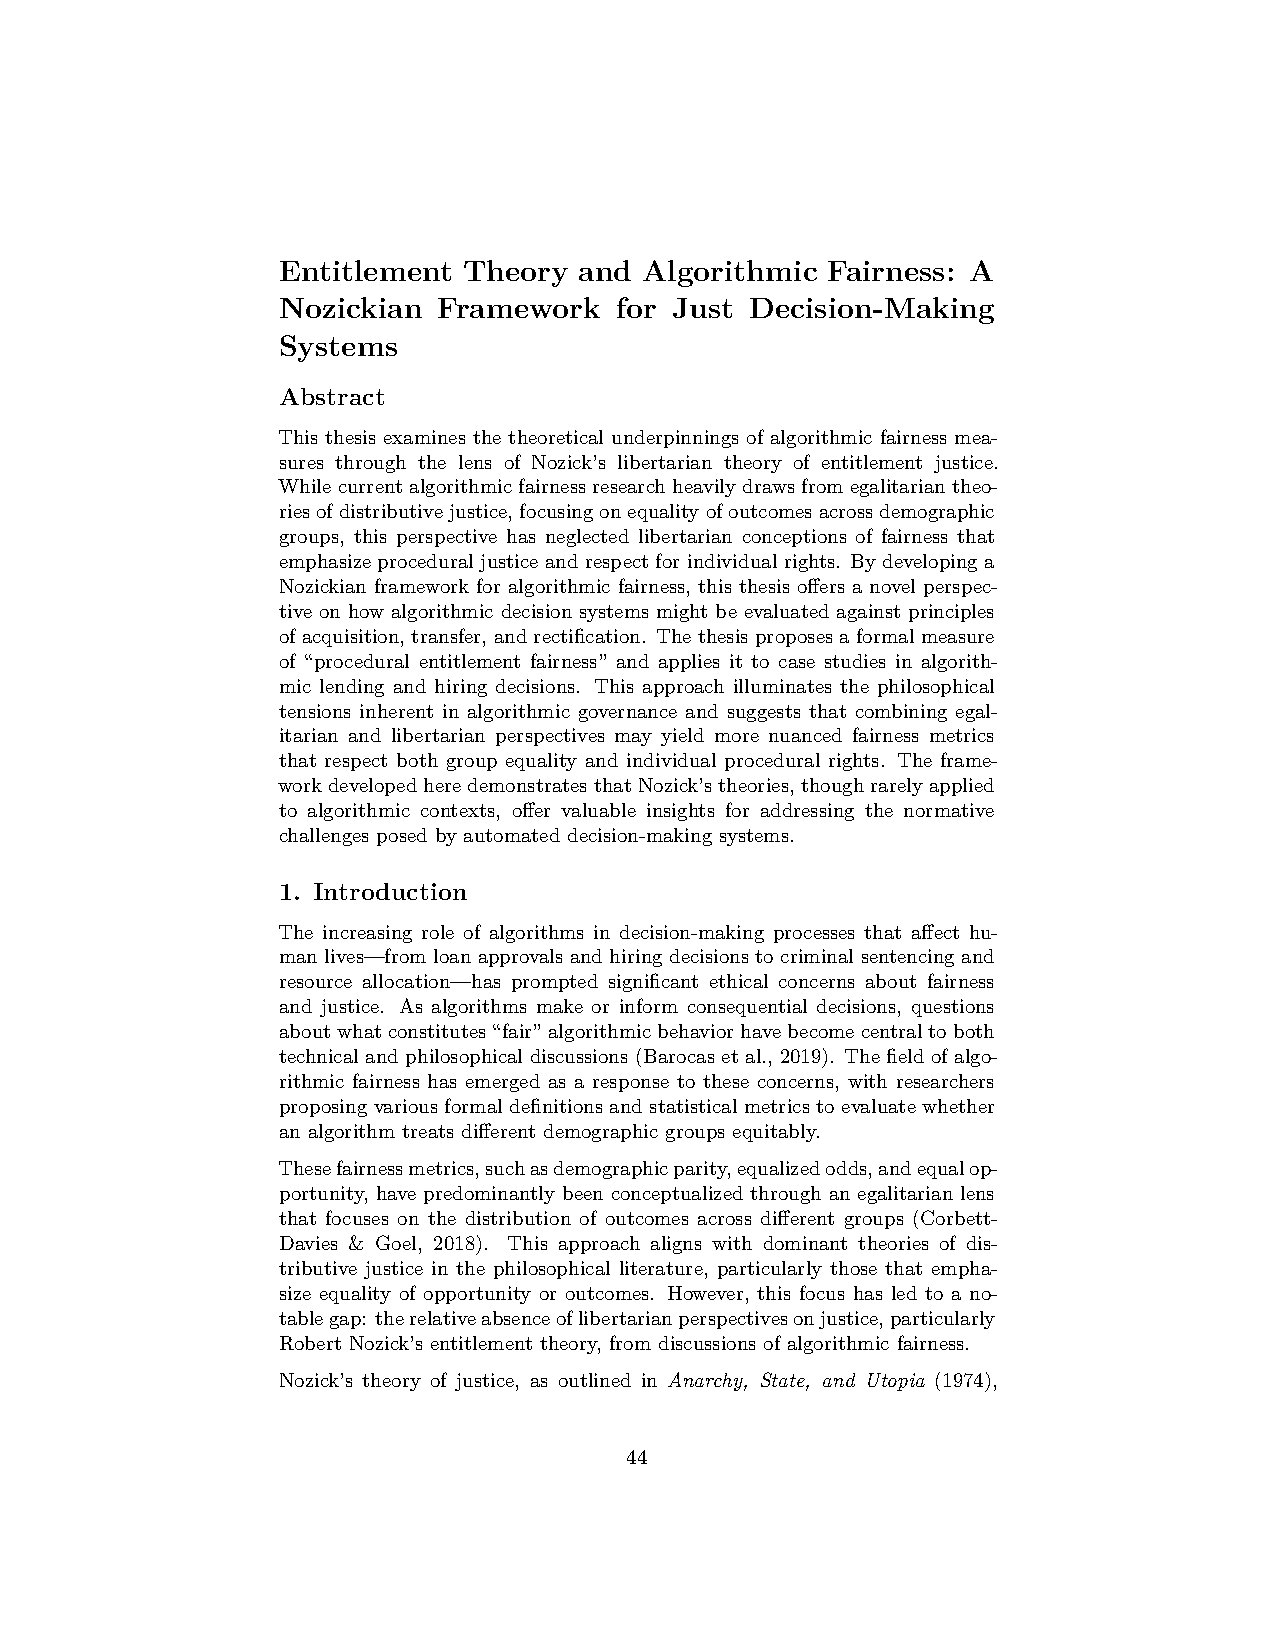
\includepdf[pages=-]{../paper_gen/gen.pdf}

\subsection{Commentary}

What follows is fully human-written text, analyzing the fully AI-generated paper
produced by Claude 3 Opus.

The paper produced by Clause 3 Opus has a few issues with structure and
mechanics, but certainly nothing that would be difficult to fix. Some of the DOI
addresses are not correct, and one of the citations given has the wrong title
of the paper. The writing style in the paper is clunky and makes use of far too
many different small sections of text, which makes it unappealing to read. 
However, these are small issues that could be fixed with a few rounds of editing
after the paper was generated—there are far more serious issues that prevent
this paper from being a viable academic work.

The paper begins relatively strongly, with a clear introduction and an accurate
presentation of the problem. The background material on algorithmic fairness and
distributive is presented clearly and correctly, and the model does a good job
of connecting to and using relevant literature. The model also does a good job
of foreshadowing an eventual argument throughout the early sections of the
paper, though the argument itself will not live up to the expectations set by
the introduction. In other words: the model does a good job of writing a viable
start to the paper, all the way up until the point where it is meant to present
a novel argument.

In leading up to a positive account of entitlement fairness, the model extracts
a lot of similar significant features to what were extracted in our paper.
Notably, the model identified that for entitlement fairness, the model must make
determinations based on the actions and decisions of individuals as a matter of
procedural justice, and must be transparent about what the actions and decisions
used are, just as we identified that that positive and negative entitlement 
features should be the basis of the decision and must be made transparent.
Similarly, the model points out that there must be a rectification procedure
through which individuals can appeal the decisions of the algorithm. The
identification and coherent defense of the relevance of these features is, 
however, followed by a main argument which is lacking in substance and clarity.

When the algorithm attempts to provide a positive account of entitlement
fairness, the argument falls flat. We are provided with a measure which is the
average of a certain score which is computed over all individuals in for whom 
decisions are made. The score contains 7 free parameters used as weights in 
linear equations, and the model provides no account of how those weights should
be set. Even if the weights were defended, the terms that are being weighted are
meaningless. For example, we are told that one of the weighted factors in the
``consent and transparency index'' is $T_i$, which is ``a measure of the 
transparency of the algorithm's decision process for individual $i$, normalized
to a value between 0 and 1.'' How is one meant to measure transparency? Why 
would transparency of one algorithm differ over different individuals? Similarly
$A$ is ``a measure of the algorithm's accessibility to contestation and appeal, 
normalized to a value between 0 and 1.'' How is this meant to be measured? 
What factors are used to compute this value? The model makes no attempt to 
address or acknowledge these questions. 

What we are left with is what you might have expected—the tone, and style of a
viable academic paper, with accurate background information and quality
structure, but with an extremely weak argument which is not well defended. Note 
that this aligns well with what was observed in the writing of our paper—Llama
did really well on background research tasks, and in determining the structure
of the paper, but was lacking in its ability to construct an original argument.
